\section{Modelos}

Ahora, lo que buscamos es construir un modelo de regresión capaz de predecir la incidencia delictiva mensual
a nivel estatal en México, utilizando como variables predictoras la entidad federativa, el bien jurídico
afectado, el tipo y subtipo de delito, la modalidad y \emph{features} temporales (año, mes, trimestre).

Para esto utilizaremos un \textbf{Random Forest Regressor} dentro de un pipeline de scikit-learn que incluye lo
siguiente:

\begin{itemize}
  \item \textbf{Preprocesamiento}: codificación One-Hot de variables categóricas y estandarización de variables
  numéricas.
  \item \textbf{Búsqueda de hiperparámetros}: Usaremos \texttt{RandomizedSearchCV} con validación cruzada de 3 pliegues,
  más eficiente que una búsqueda exhaustiva para este volumen de datos.
  \item \textbf{Transformación del objetivo}: Aplicaremos \texttt{log1p} a la variable objetivo para mitigar el sesgo
  observado en el EDA.
\end{itemize}

El dataset contiene $\sim$414,000 registros de incidencia delictiva estatal, por lo que trabajar con todos
estos registros es demasiado pesado en recursos. Es por esto que para este modelo trabajaremos con una
muestra estratificada de 50,000 registros que preserva la proporción de tipos de delito.

El cuaderno de Jupyter Notebook que acompaña esta sección se encuentra disponible haciendo click
\href{https://github.com/wallsified/proyecto-final-aymdd/blob/main/notebooks/models.ipynb}{aquí}.

\begin{lstlisting}[language=Python, caption={Carga de librerías y módulos del proyecto}, label={lst:carga-modelos}]
import sys
from pathlib import Path

sys.path.insert(0, str(Path.cwd().parent))

import pandas as pd
import numpy as np
import matplotlib.pyplot as plt
import seaborn as sns

from sklearn.model_selection import train_test_split

from src.model.preprocesamiento import (
    cargar_preparar_datos,
    separar_features_target,
    construir_preprocesador,
)
from src.model.entrenamiento import entrenar_random_forest
from src.model.evaluacion import evaluar_modelo, grafica_predicciones, grafica_residuales
from src.model.persistencia import guardar_modelo

pd.set_option("display.max_columns", 20)
pd.set_option("display.width", 140)
\end{lstlisting}

\subsection{Carga y preparación de datos}

Cargamos el dataset limpio resultado del EDA y aplicamos un muestreo estratificado sobre la columna
\texttt{tipo\_delito} para reducir los $\sim$414,000 registros a 50,000. Esto preserva la distribución de tipos de
delito y reduce drásticamente el tiempo de entrenamiento sin comprometer la calidad del modelo, ya que
Random Forest muestra rendimientos decrecientes con volúmenes de datos muy grandes.

Luego, separamos las features de nuestra variable objetivo: \texttt{incidencia\_delictiva}, y aplicamos una
transformación logarítmica con \texttt{log1p} para compensar el fuerte sesgo a la derecha observado en el EDA.

\begin{lstlisting}[language=Python, caption={Carga y muestra estratificada del dataset}, label={lst:carga-datos-modelo}]
RUTA_DATOS = str(Path.cwd().parent / "data" / "processed" / "INM_estatal_dic25_clean.csv")

df = cargar_preparar_datos(RUTA_DATOS)
print(f"Muestra estratificada: {df.shape[0]:,} filas x {df.shape[1]} columnas")
df.head(3)
\end{lstlisting}

\begin{lstlisting}
Muestra estratificada: 50,000 filas x 7 columnas
\end{lstlisting}

\begin{table}[ht]
  \centering
  \caption{Primeras filas del dataset muestreado}
  \resizebox{\textwidth}{!}{%
    \begin{tabular}{l l l l l l l l}
      \hline
      \textbf{idx} & \textbf{fecha} & \textbf{entidad} & \textbf{bien\_juridico\_afectado} & \textbf{tipo\_delito} & \textbf{subtipo\_delito} & \textbf{modalidad} & \textbf{incidencia\_delictiva} \\
      \hline
      249379 & 2021-03-01 & Puebla & El patrimonio & Otros delitos contra el patrimonio & Otros delitos contra el patrimonio & Otros delitos contra el patrimonio & 26 \\
      57395 & 2016-09-01 & Morelos & La vida y la Integridad corporal & Lesiones & Lesiones dolosas & No especificado & 144 \\
      289658 & 2022-12-01 & Quintana Roo & El patrimonio & Robo & Robo de vehículo automotor & Robo de coche de 4 ruedas Con violencia & 11 \\
    \end{tabular}%
  }
  \label{tab:primeras-filas-modelo}
\end{table}

La columna \texttt{fecha}, al ser de tipo datetime, se descompone en tres features numéricas: \texttt{anio}, \texttt{mes} y
\texttt{trimestre}. Esto permite al modelo capturar tendencias temporales (tendencia anual, estacionalidad mensual
y patrones por trimestre) sin introducir alta cardinalidad como haría un One-Hot de fechas individuales.

\begin{lstlisting}[language=Python, caption={Separación de features y target con transformación log1p}, label={lst:features-target}]
X, y = separar_features_target(df)

print(f"Features: {X.shape[1]} columnas")
print(f"Columnas: {list(X.columns)}")
print(f"\nTarget (log1p) - media: {y.mean():.3f}, std: {y.std():.3f}")
X.head(3)
\end{lstlisting}

\begin{lstlisting}
Features: 8 columnas
Columnas: ['entidad', 'bien_juridico_afectado', 'tipo_delito', 'subtipo_delito', 'modalidad', 'anio', 'mes', 'trimestre']

Target (log1p) - media: 1.753, std: 1.990
\end{lstlisting}

\begin{table}[ht]
  \centering
  \caption{Primeras filas de las features (X) y el target transformado (y)}
  \resizebox{\textwidth}{!}{%
    \begin{tabular}{l l l l l l l l l}
      \hline
      \textbf{idx} & \textbf{entidad} & \textbf{bien\_juridico\_afectado} & \textbf{tipo\_delito} & \textbf{subtipo\_delito} & \textbf{modalidad} & \textbf{anio} & \textbf{mes} & \textbf{trimestre} \\
      \hline
      249379 & Puebla & El patrimonio & Otros delitos contra el patrimonio & Otros delitos contra el patrimonio & Otros delitos contra el patrimonio & 2021 & 3 & 1\\
      57395 & Morelos & La vida y la Integridad corporal & Lesiones & Lesiones dolosas & No especificado & 2016 & 9 & 3\\
      289658 & Quintana Roo & El patrimonio & Robo & Robo de vehículo automotor & Robo de coche de 4 ruedas Con violencia & 2022 & 12 & 4 \\
      \hline
    \end{tabular}%
  }
  \label{tab:features-target}
\end{table}


\subsection{Preprocesamiento y división train/test}

Separamos el 80\% de los datos para entrenamiento y el 20\% restante para prueba, con una semilla fija para
reproducibilidad.

El preprocesador aplica dos transformaciones dentro del pipeline:

\begin{itemize}
  \item \textbf{OneHotEncoder} sobre las columnas categóricas (\texttt{entidad}, \texttt{bien\_juridico\_afectado}, \texttt{tipo\_delito},
  \texttt{subtipo\_delito}, \texttt{modalidad}). Esto para convertir cada categoría en una columna binaria. Se configura
  \texttt{handle\_unknown="ignore"} para que no falle si aparece una categoría nueva en el conjunto de prueba.
  \item \textbf{StandardScaler} sobre las columnas numéricas (\texttt{anio}, \texttt{mes}, \texttt{trimestre}) para estandarizar la
  media 0 y la desviación a 1.
\end{itemize}

Al integrar el preprocesador dentro del \texttt{Pipeline}, se evita el \textbf{data leakage}, pues así el
\texttt{OneHotEncoder} y el \texttt{StandardScaler} se ajustan únicamente sobre los datos de entrenamiento en cada
pliegue de la validación cruzada.

\begin{lstlisting}[language=Python, caption={Construcción del preprocesador y división train/test}, label={lst:preprocesador-split}]
preprocessor = construir_preprocesador(X)

X_train, X_test, y_train, y_test = train_test_split(
    X, y, test_size=0.20, random_state=42
)

print(f"Train: {X_train.shape[0]:,} filas")
print(f"Test:  {X_test.shape[0]:,} filas")
\end{lstlisting}

\begin{lstlisting}
Train: 40,000 filas
Test:  10,000 filas
\end{lstlisting}

\subsection{Entrenamiento del modelo}

Utilizamos \textbf{\texttt{RandomizedSearchCV}} para buscar los mejores hiperparámetros del Random Forest.
La razón principal por la que ocupamos esto y no \texttt{GridSearchCV} es porque el segundo evalúa todas
las combinaciones posibles, mientras que el primero muestrea un número fijo de combinaciones aleatorias,
lo que resulta más eficiente con datasets grandes como lo es el nuestro.

Ocuparemos el siguiente espacio de búsqueda:

\begin{table}[ht]
 \centering
  \caption{Espacio de búsqueda de hiperparámetros}
    \begin{tabular}{l l}
      \hline
      \textbf{Parámetro} & \textbf{Valores} \\
      \hline
      \texttt{n\_estimators} & 100, 150 \\
      \texttt{max\_depth} & 15, None (sin límite) \\
      \texttt{min\_samples\_split} & 2, 5 \\
      \hline
    \end{tabular}
  \label{tab:hyperparametros}
\end{table}

junto a la siguiente configuración (la cual está hardcodeada en \texttt{src/model/entrenamiento.py}):
\begin{itemize}
  \item \texttt{n\_iter=8}: evalúa 8 combinaciones aleatorias de los parámetros.
  \item \texttt{cv=3}: validación cruzada con 3 pliegues.
  \item \texttt{scoring='r2'}: optimiza el coeficiente de determinación R$^2$.
  \item \texttt{n\_jobs=-1}: utiliza todos los núcleos disponibles del procesador.
\end{itemize}

\begin{lstlisting}[language=Python, caption={Entrenamiento con RandomizedSearchCV}, label={lst:entrenamiento-rf}]
search = entrenar_random_forest(X_train, y_train, preprocessor)

print(f"Mejores parámetros: {search.best_params_}")
print(f"Mejor R² (CV):      {search.best_score_:.4f}")
\end{lstlisting}

\begin{lstlisting}
Fitting 3 folds for each of 8 candidates, totalling 24 fits
Mejores parámetros: {'model__n_estimators': 150, 'model__min_samples_split': 2, 'model__max_depth': None}
Mejor R² (CV):      0.9201
\end{lstlisting}

\subsection{Evaluación del modelo}

Evaluamos el rendimiento del mejor modelo sobre el conjunto de \textbf{prueba} (20\% de los datos, no
utilizado en el entrenamiento ni en la búsqueda de hiperparámetros) en base a las siguientes métricas:

\begin{itemize}
  \item \textbf{MAE} (Error Absoluto Medio): error promedio en las mismas unidades que el target (escala log). Un
  valor de 0.38 indica que, en promedio, la predicción se desvía $\sim$0.38 unidades logarítmicas del valor real.
  \item \textbf{MSE} (Error Cuadrático Medio): penaliza más los errores grandes.
  \item \textbf{RMSE} (Raíz del Error Cuadrático Medio): en la misma escala que el target, más interpretable que el MSE.
  \item \textbf{R$^2$} (Coeficiente de Determinación): proporción de la varianza explicada por el modelo. Un valor de
  1.0 es predicción perfecta; 0.0 equivale a predecir siempre la media.
\end{itemize}

\begin{lstlisting}[language=Python, caption={Evaluación del modelo en el conjunto de prueba}, label={lst:evaluacion-modelo}]
mejor_modelo = search.best_estimator_

metricas, y_pred = evaluar_modelo(mejor_modelo, X_test, y_test)
display(metricas)
\end{lstlisting}

\begin{table}[ht]
  \centering
  \caption{Métricas de evaluación del modelo en el conjunto de prueba}
    \begin{tabular}{l l}
      \hline
      MAE & 0.307301\\
      MSE & 0.262411\\
      RMSE & 0.512261\\
      R2 & 0.932790\\
      \hline
    \end{tabular}
  \label{tab:metricas-evaluacion}
\end{table}

\subsubsection{Importancia de features}

El Random Forest permite extraer la \textbf{importancia} de cada feature, medida por cuánto reduce la impureza
de los nodos del árbol. Dado que las 5 columnas categóricas fueron codificadas con One-Hot (generando cientos
de columnas binarias), agrupamos la importancia por columna original para obtener una visión interpretable de
qué variables son las que más contribuyen a las predicciones.

\begin{lstlisting}[language=Python, caption={Cálculo y visualización de importancia de features}, label={lst:importancia-features}]
preprocessor = mejor_modelo.named_steps["preprocessor"]
feature_names = mejor_modelo[:-1].get_feature_names_out()
importances = mejor_modelo[-1].feature_importances_

cat_cols = [t[2] for t in preprocessor.transformers_ if t[0] == "cat"][0]
num_cols = [t[2] for t in preprocessor.transformers_ if t[0] == "num"][0]

def agrupar_feature(nombre):
    if nombre.startswith("num__"):
        return nombre[5:]
    codificado = nombre[5:]
    for col in cat_cols:
        if codificado.startswith(col + "_"):
            return col
    return codificado

importance_df = pd.DataFrame({
    "feature": feature_names,
    "importance": importances
})
importance_df["grupo"] = importance_df["feature"].apply(agrupar_feature)

importancia_por_grupo = (
    importance_df.groupby("grupo")["importance"]
    .sum()
    .sort_values(ascending=True)
)

plt.figure(figsize=(10, 6))
importancia_por_grupo.plot(kind="barh", color="steelblue")
plt.xlabel("Importancia acumulada")
plt.title("Importancia de features (agrupada por columna original)")
plt.tight_layout()
plt.show()
\end{lstlisting}


\begin{figure}[H]
  \centering
  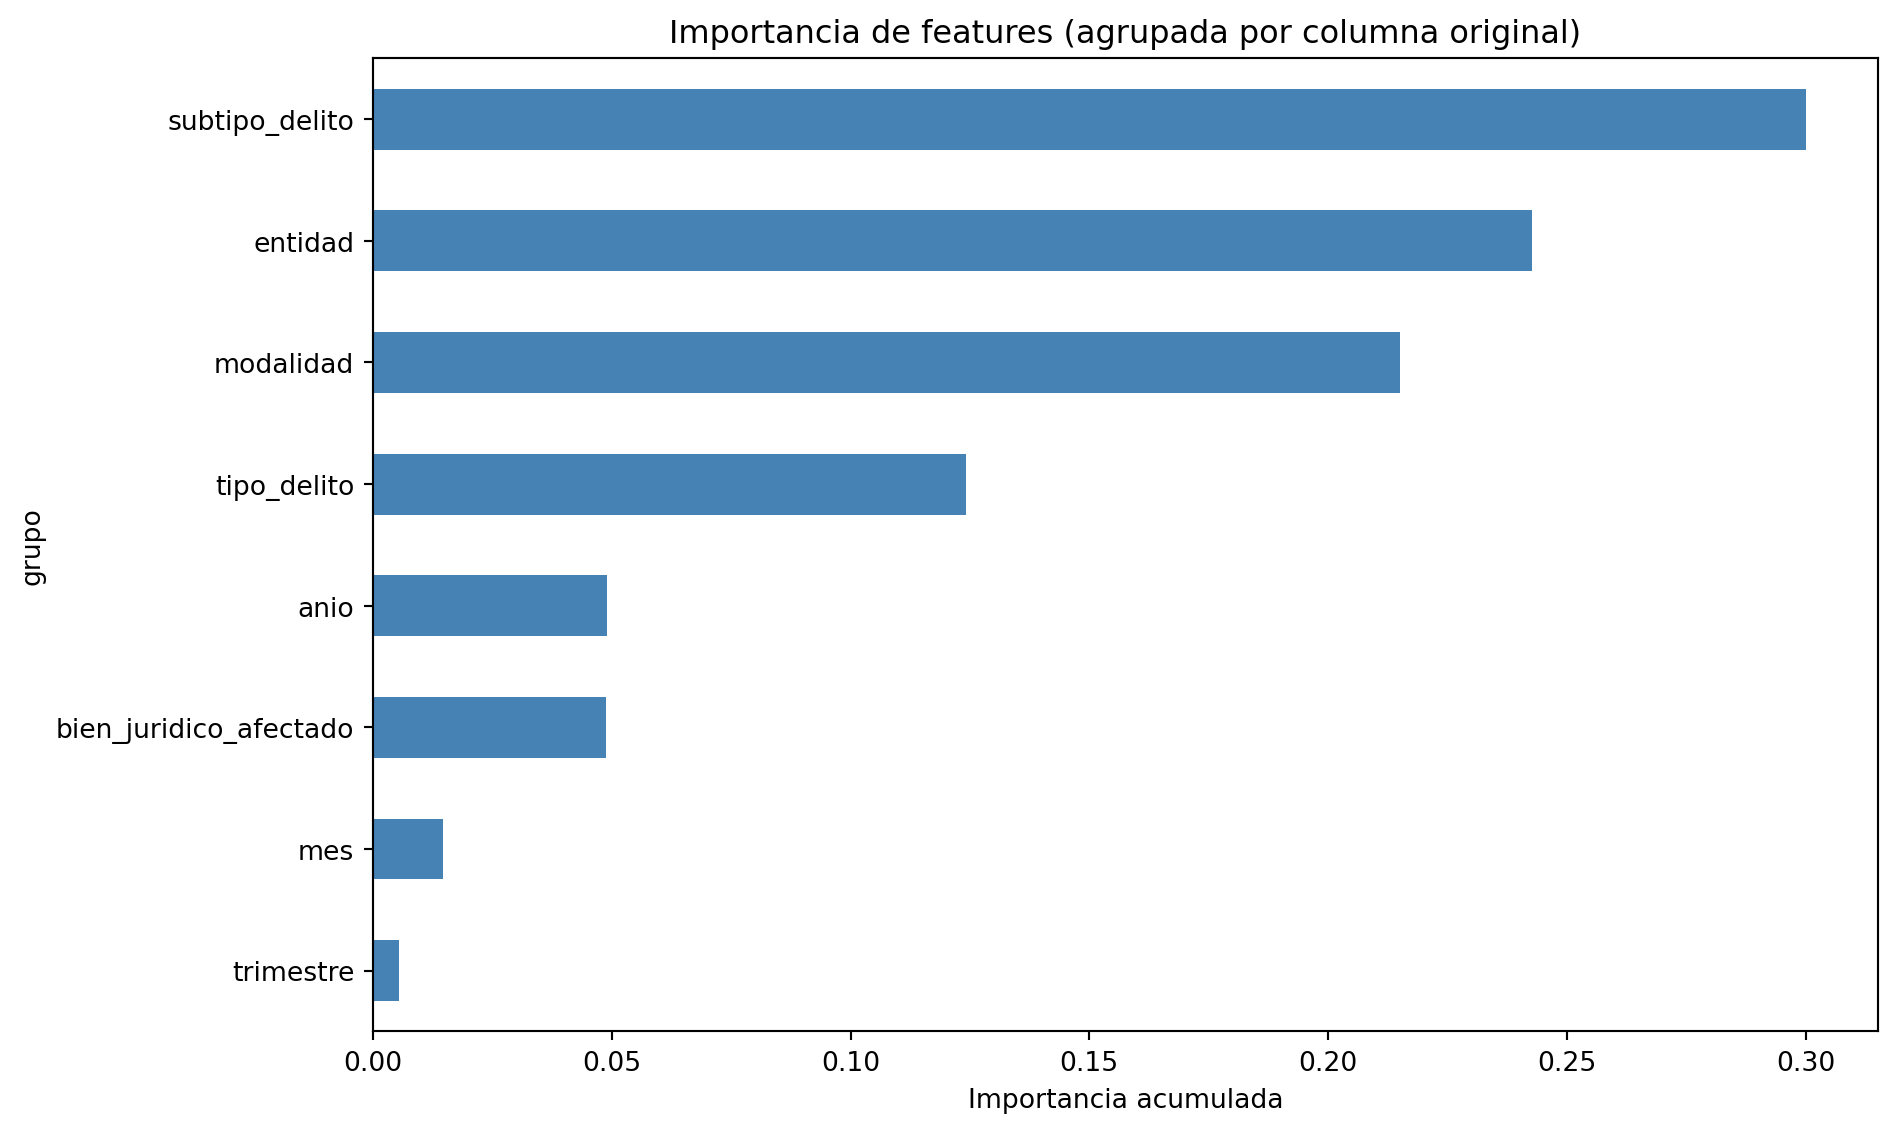
\includegraphics[width=0.75\textwidth]{imagenes/features-importance.png}
  \caption{Importancia de features agrupada por columna original}
  \label{fig:importancia-features}
\end{figure}

\subsection{Interpretación del Modelo}

El modelo obtenido tiene las siguientes implicaciones:

\begin{itemize}

\item \textbf{R$^2$ = 0.93 --- Alta capacidad predictiva.} El 93\% de la variación en la incidencia delictiva se explica por
la combinación de entidad federativa, clasificación delictiva y variables temporales. Esto indica que el
delito en México \textbf{no es un fenómeno aleatorio}: sigue patrones sistemáticos y repetibles que el modelo
puede capturar.

\item \textbf{Patrones geográficos.} Cada entidad federativa tiene un ``perfil delictivo'' distintivo. Estados como
CDMX, Estado de México y Jalisco concentran volúmenes altos en ciertas categorías, mientras que estados
como Colima o Tlaxcala muestran otras dinámicas. La feature \texttt{entidad} captura estas diferencias estructurales.

\item \textbf{Patrones por clasificación delictiva.} La jerarquía \texttt{bien\_juridico} $\rightarrow$ \texttt{tipo} $\rightarrow$ \texttt{subtipo} $\rightarrow$ \texttt{modalidad} permite
al modelo distinguir entre categorías con volúmenes muy dispares. Por ejemplo, ``homicidio'' tiene incidencias
bajas mientras que ``robo'' tiene incidencias altas; la modalidad (con/sin violencia) añade granularidad
adicional.

\item \textbf{Patrones temporales.} Las features \texttt{anio}, \texttt{mes} y \texttt{trimestre} capturan:
    \begin{itemize}
    \item \textbf{Tendencia}: incrementos o disminuciones sostenidos a lo largo de los años.
    \item \textbf{Estacionalidad}: ciclos mensuales o trimestrales (por ejemplo, incrementos en diciembre por
    temporadas vacacionales).
    \end{itemize}

\item \textbf{MAE $\approx$ 0.31 en escala log.} Para interpretar en unidades originales: $\exp(0.31) \approx 1.36$, lo que significa
que el error promedio de predicción es de aproximadamente \textbf{36\% sobre el valor real}. Para un dataset con
valores que van de decenas a miles de incidentes, esto es un margen de error razonable.

\end{itemize}

\subsubsection{Análisis gráfico}

Las gráficas de \textbf{Real vs Predicho} y de \textbf{residuales} permiten evaluar visualmente la calidad del ajuste.
En un buen modelo, los puntos deben agruparse alrededor de la diagonal en la primera gráfica, y los residuales
deben distribuirse simétricamente alrededor de cero en la segunda.

\begin{lstlisting}[language=Python, caption={Gráficas de predicciones y residuales}, label={lst:graficas-evaluacion}]
grafica_predicciones(y_test, y_pred)
grafica_residuales(y_test, y_pred)
\end{lstlisting}

\begin{figure}[H]
  \centering
  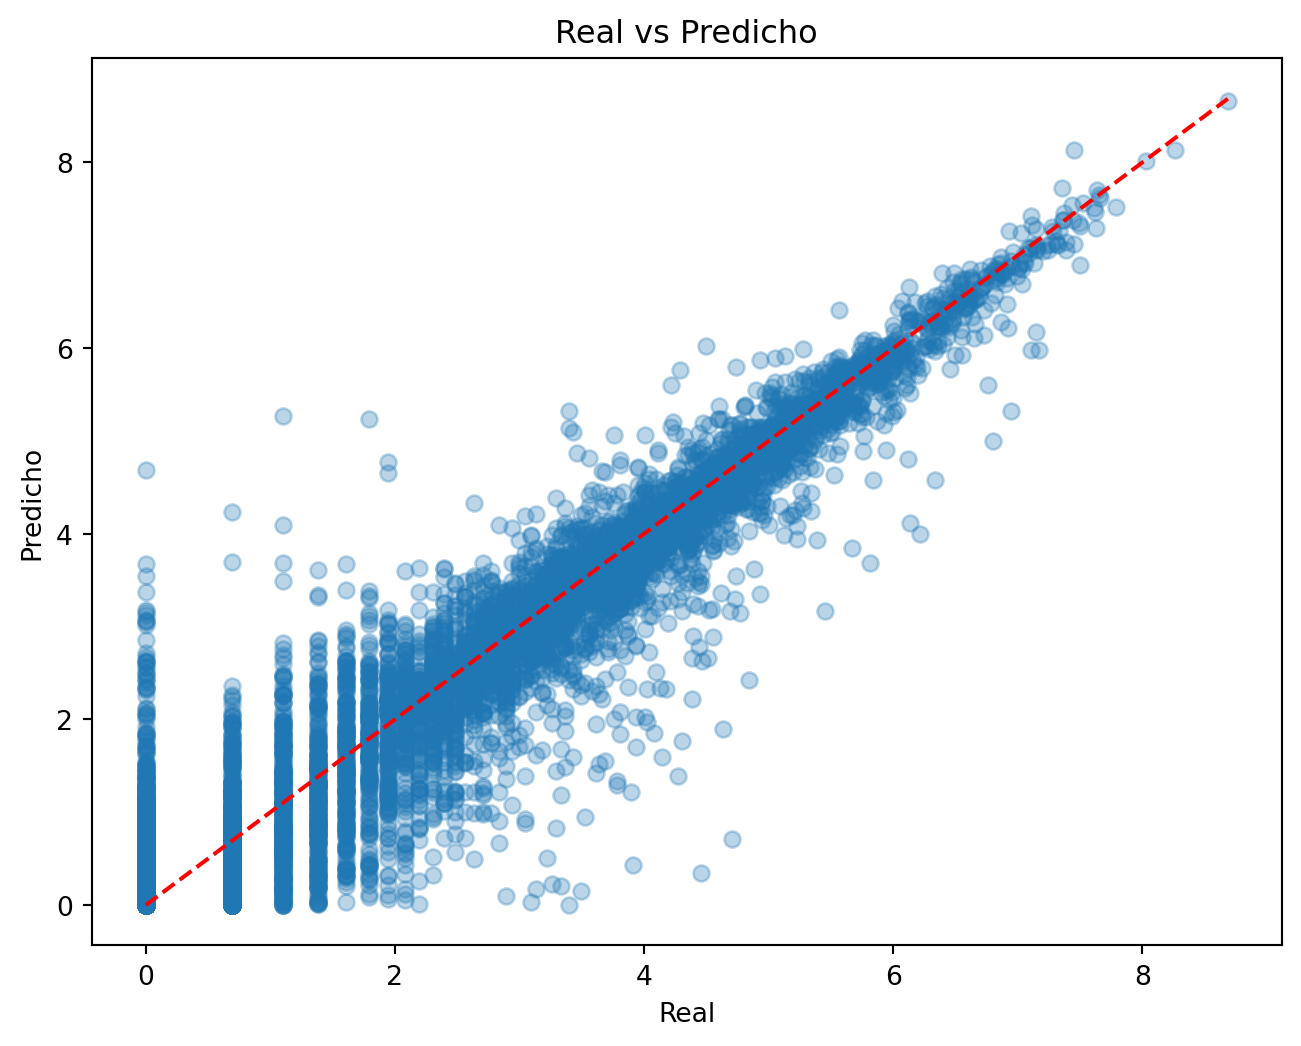
\includegraphics[width=0.7\textwidth]{imagenes/real-presaid.png}
  \caption{Gráfica de Real vs Predicho}
  \label{fig:real-vs-predicho}
\end{figure}

\begin{figure}[H]
  \centering
  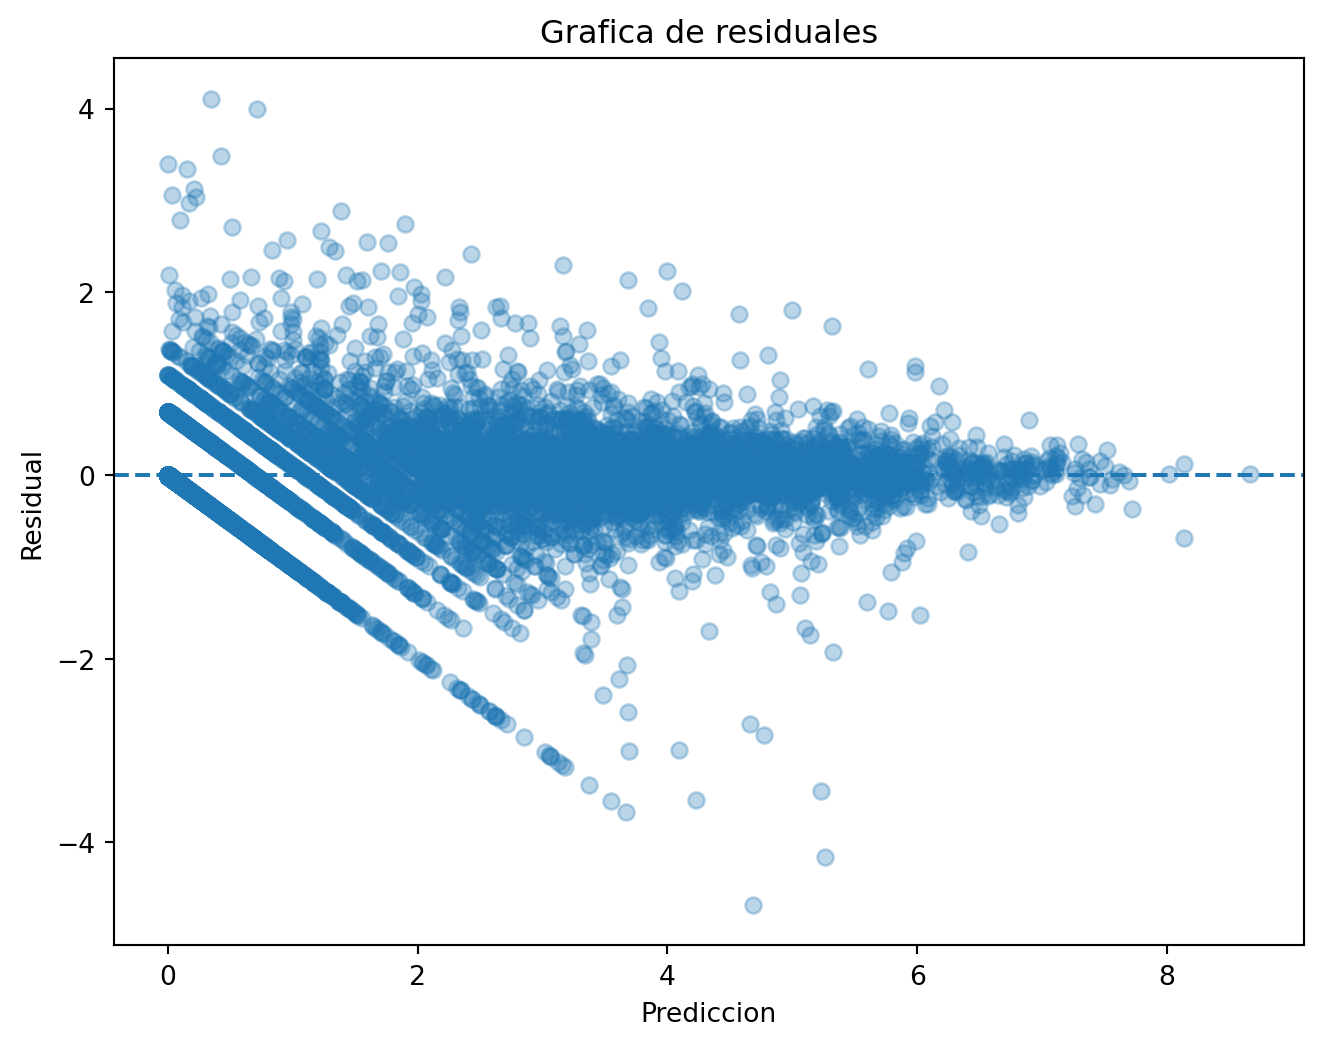
\includegraphics[width=0.7\textwidth]{imagenes/residuals.png}
  \caption{Gráfica de residuales del modelo}
  \label{fig:residuales}
\end{figure}

\subsection{Comparación con Línea Base}

Para verificar que el modelo aporta valor real, lo comparamos contra un \textbf{DummyRegressor} que simplemente
predice la media del target en cada caso. Si el Random Forest no supera significativamente a este modelo
trivial, significaría que las features elegidas no tienen poder predictivo.

\begin{lstlisting}[language=Python, caption={Comparación con DummyRegressor como línea base}, label={lst:linea-base}]
from sklearn.dummy import DummyRegressor
from sklearn.pipeline import Pipeline

baseline = Pipeline([
    ("preprocessor", preprocessor),
    ("model", DummyRegressor(strategy="mean"))
])

baseline.fit(X_train, y_train)

baseline_metricas, _ = evaluar_modelo(baseline, X_test, y_test)
display(baseline_metricas)
\end{lstlisting}

\begin{table}[ht]
  \centering
  \caption{Métricas del DummyRegressor (línea base)}
    \begin{tabular}{l l}
      \hline
      MAE & 1.719015\\
      MSE & 3.904472\\
      RMSE & 3.904472\\
      R2 & -0.000034\\
      \hline
    \end{tabular}
  \label{tab:dummy-metricas}
\end{table}

El DummyRegressor obtiene un R$^2$ $\approx$ 0 (como es esperado, ya que predecir la media no explica variación).
El Random Forest, con un R$^2$ significativamente mayor, demuestra que las features utilizadas capturan
patrones reales de la incidencia delictiva.

\subsection{Persistencia del modelo}

Finalmente, guardamos el modelo entrenado en un archivo \texttt{.joblib} para su uso futuro en predicciones o análisis
adicionales. Debido al peso del modelo final este se puede descargar desde
\href{https://drive.google.com/file/d/1p3M8-Q3r0L0FgIDpoM59of0usDTnXWrY/view?usp=sharing}{aquí}
para evitar problemas de espacio en el repositorio y de ésta página.

Sin embargo, la instrucción para guardar el modelo es la siguiente:

\begin{lstlisting}[language=Python, caption={Guardado del modelo entrenado}, label={lst:guardar-modelo}]
guardar_modelo(mejor_modelo, "../models/modelo_incidencia_delictiva.joblib")
\end{lstlisting}

\subsection{Ejemplo de Predicción}
Ahora intentaremos predecir los valores en base al modelo. Queremos predecir la incidencia delictiva de los
siguientes casos:

\begin{table}[ht]
  \centering
  \caption{Ejemplo de datos de entrada para predicción de incidencia delictiva}
  \label{tab:datos_prediccion}
  \resizebox{\textwidth}{!}{%
  \begin{tabular}{|l|l|l|l|l|c|c|c|}
    \hline
    \textbf{Entidad} & \textbf{Bien jurídico} & \textbf{Tipo de delito} & \textbf{Subtipo de delito} & \textbf{Modalidad} & \textbf{Año} & \textbf{Mes} & \textbf{Trimestre} \\ \hline
    Ciudad de México & El patrimonio & Robo & Robo de vehiculo automotor & Robo de coche de 4 ruedas Con violencia & 2026 & 5 & 1 \\ \hline
    Jalisco & La vida y la Integridad corporal & Homicidio & Homicidio doloso & Con arma de fuego & 2026 & 5 & 1 \\ \hline
  \end{tabular}%
  }
\end{table}


\begin{lstlisting}
modelo = cargar_modelo("../models/modelo_incidencia_delictiva.joblib")

# Preparación de los datos de entrada
# Las features deben coincidir con las usadas en el entrenamiento:
# - Categóricas: entidad, bien_juridico_afectado, tipo_delito, subtipo_delito, modalidad
# - Numéricas: anio, mes, trimestre

datos_ejemplo = pd.DataFrame({
    "entidad": ["Ciudad de México", "Jalisco"],
    "bien_juridico_afectado": ["El patrimonio", "La vida y la Integridad corporal"],
    "tipo_delito": ["Robo", "Homicidio"],
    "subtipo_delito": ["Robo de vehiculo automotor", "Homicidio doloso"],
    "modalidad": ["Robo de coche de 4 ruedas Con violencia", "Con arma de fuego"],
    "anio": [2026, 2026],
    "mes": [5, 5],
    "trimestre": [1, 1]
})


# El modelo predice en escala logarítmica (log1p), por lo que debemos invertir la transformación
predicciones_log = modelo.predict(datos_ejemplo)
predicciones = np.expm1(predicciones_log)  # Inversión de log1p

resultados = datos_ejemplo.copy()
resultados["incidencia_predicha"] = predicciones.round(0).astype(int)

print("Predicciones de incidencia delictiva:")
resultados
\end{lstlisting}

\begin{table}[ht]
  \centering
  \caption{Predicciones de incidencia delictiva para los casos de ejemplo}
  \label{tab:predicciones-ejemplo}
  \resizebox{\textwidth}{!}{%
  \begin{tabular}{|l|l|l|l|l|l|c|c|c|c|}
    \hline
    \textbf{Entidad} & \textbf{Bien jurídico} & \textbf{Tipo de delito} & \textbf{Subtipo de delito} & \textbf{Modalidad} & \textbf{Año} & \textbf{Mes} & \textbf{Trimestre} & \textbf{Incidencia predicha} \\ \hline
    Ciudad de México & El patrimonio & Robo & Robo de vehiculo automotor & Robo de coche de 4 ruedas Con violencia & 2026 & 5 & 1 & 50 \\ \hline
    Jalisco & La vida y la Integridad corporal & Homicidio & Homicidio doloso & Con arma de fuego & 2026 & 5 & 1 & 61 \\ \hline
  \end{tabular}%
  }
\end{table}


\subsection{Conclusiones sobre el modelo}

El modelo de Random Forest logra predecir la incidencia delictiva estatal mensual con un R$^2$ de 0.93, superando
ampliamente a la línea base (R$^2$ $\approx$ 0). Esto confirma que:

\begin{enumerate}
  \item La incidencia delictiva en México está fuertemente determinada por la ubicación geográfica, el tipo de
  delito y el momento en el tiempo. El 93\% de la variación en la incidencia delictiva se explica por la
  combinación de ubicación geográfica, clasificación delictiva y momento en el tiempo. Esto descarta la
  hipótesis de que la criminalidad sea un fenómeno aleatorio o caótico: sigue patrones estables y recurrentes
  que un modelo de aprendizaje automático puede capturar con alta precisión.

  \item Las variables utilizadas (entidad, clasificación delictiva, año/mes/trimestre) son suficientes para
  construir un modelo predictivo robusto. Sobre todo con estos datos más recientes, ya que el EDA mostró que
  la incidencia delictiva no ha decrecido entre 2015 y 2025, con un incremento notable desde 2022. Además,
  se observa estacionalidad: los picos se concentran entre marzo y junio en los últimos años (antes eran
  mayo-agosto). El modelo captura estos ciclos a través de las features \texttt{anio}, \texttt{mes} y \texttt{trimestre}, lo
  que permite identificar cuándo ocurren los periodos de mayor riesgo.

  \item Los patrones delictivos son \textbf{estables y predecibles} en condiciones normales, lo cual es relevante
  para la planeación de políticas de seguridad. En particular, la clasificación delictiva es el predictor
  más potente, ya que la jerarquía \texttt{bien\_juridico} $\rightarrow$ \texttt{tipo} $\rightarrow$ \texttt{subtipo} $\rightarrow$ \texttt{modalidad} permite distinguir entre
  categorías con volúmenes drásticamente diferentes. Como se vio en el EDA, Robo es el delito más reportado,
  pero la modalidad (con violencia, sin violencia, de vehículo automotor, etc.) añade granularidad que el
  modelo aprovecha para hacer predicciones más precisas.
\end{enumerate}

\subsubsection{Limitaciones}

\begin{itemize}
  \item El modelo aprende patrones históricos y no puede predecir anomalías como pandemias, crisis o cambios de
  política pública. El caso de 2020 (valores inusualmente bajos por COVID-19) es un ejemplo de evento que
  el modelo no anticiparía.
  \item Los datos dependen de denuncias ante el Ministerio Público, por lo que zonas con bajo reporte pueden tener
  valores artificialmente bajos.
  \item El modelo identifica correlaciones, no causalidades. Por ejemplo, saber que CDMX tiene alta incidencia
  de robo no explica por qué ocurre, lo cual es algo ajeno a lo que se realiza en este proyecto.
\end{itemize}
